\chapter{Design del Controllo}

Il modello del controllo scelto si basa sul DDPG (presentato nella sez. \ref{ddpgsection}). In questo capitolo ci si soffermerà sulla particolarizzazione dell'algoritmo nel caso di applicazione specifico.
\newline

L'obiettivo dell'agente, in questo caso, è quello di far rimanere sempre in carreggiata l'auto, mentre cerca di farle completare il percorso più velocemente possibile, in uno scenario ad agente singolo. 

Il modello dell'intero sistema di fig.\ref{fig:system_model} mostra le interazioni tra agente ed environment TORCS.
\newline

Il flusso del sistema può essere diviso in due parti fondamentali che avvengono simultaneamente ad ogni istante di tempo $t$:
\begin{enumerate}
    \item \textit{Esplorazione:} A partire da una osservazione $s_t$ la rete Actor $\mu_{\phi}$ produce un'azione $a_t=\mu_{\phi}(s_t)$, con $a_t=(a_{accel},a_{brake},a_{steer}) \in \mathbb{R}^3$. A questa azione viene aggiunto un \textit{rumore esplorativo} e il risultato viene poi inviato a TORCS che restituisce lo stato successivo $s_{t+1}$. Dallo stato successivo si calcola la ricompensa immediata $r_{t+1}$. La transizione del sistema $(s_t,a_t,s_{t+1},r_{t+1})$ viene infine memorizzata nell'experience replay per l'allenamento dell'agente.
    \item \textit{Allenamento:} Viene prelevato un batch di transizioni dal buffer. I parametri della rete Critic $Q_{\theta}$ vengono aggiornati seguendo la loss di eq.\ref{criticlossddpg}. L'Actor, successivamente, viene aggiornato secondo il gradiente di eq.\ref{gradactorddpg}. Infine i parametri delle reti target vengono aggiornati tramite soft update seguendo la eq.\ref{ddpgsoftupdate_eq}.
\end{enumerate}

\begin{figure}[hb]
    \center
    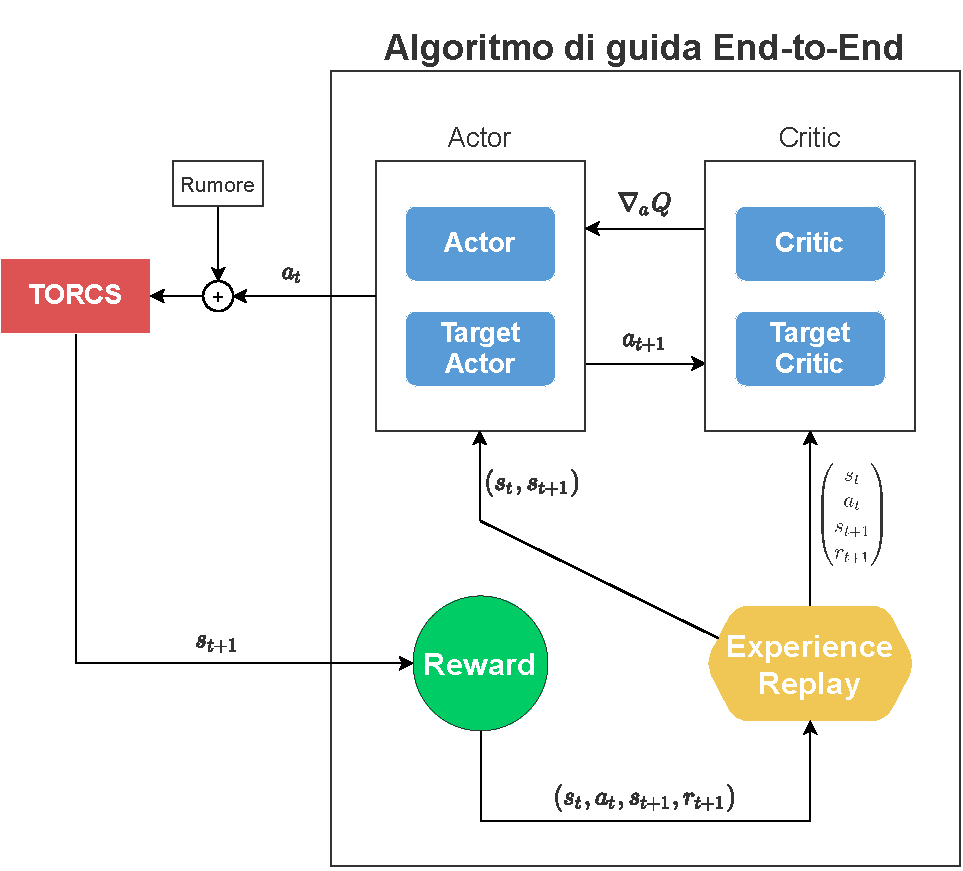
\includegraphics[width = 6in]{Figures/Chapter4/model_ddpg.drawio.pdf}
    \caption{Modello del sistema TORCS-Agente}
    \label{fig:system_model}
\end{figure}

\clearpage

\section{Architettura delle reti}

In questa sezione vengono definite le architetture delle reti utilizzate.
\newline

La rete Actor di fig.\ref{fig:actor_network} è una rete \textit{fully connected} con un input di 24 neuroni, che rappresentano lo stato, e un output di 3 neuroni, ovvero le azioni. I due neuroni che producono l'uscita di \textit{accel} e \textit{brake} sono attivati con \textit{sigmoide} per garantire un output compreso in $[0,1]$, mentre il neurone che produce l'azione di \textit{steer} viene attivato dalla \textit{tangente iperbolica} in modo da avere un range di uscita compreso in $[-1,+1]$. Frapposti tra i livelli di ingresso e uscita ci sono due livelli nascosti da 300 e 400 neuroni con attivazione relu.



\begin{figure}[hb]
    \center
    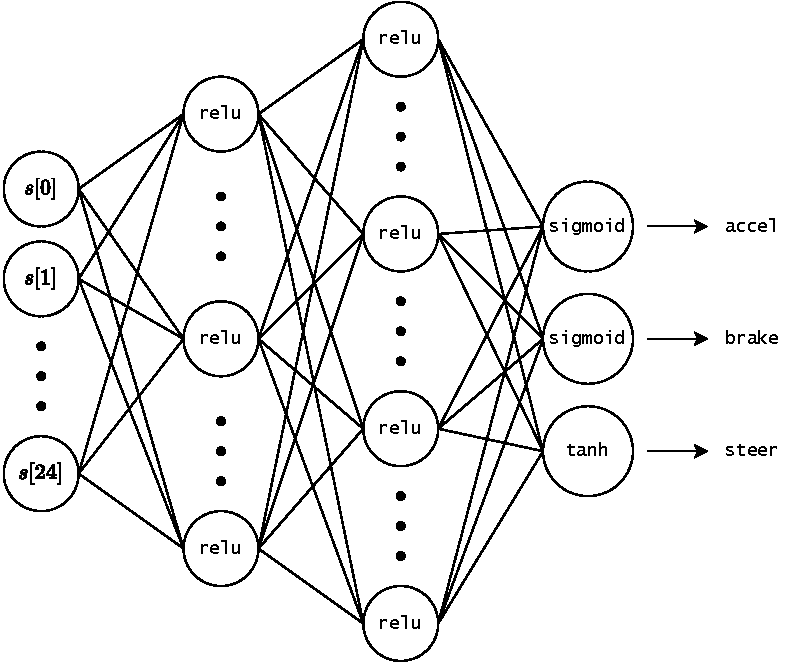
\includegraphics[width = 3.5in]{Figures/Chapter4/ddpg_actor_network.drawio.pdf}
    \caption{Rete Actor}
    \label{fig:actor_network}
\end{figure}

\clearpage

La struttura della rete Critic è mostrata in fig.\ref{fig:critic_network}. L'input è diviso in due parti, una è l'informazione sullo stato dell'ambiente fornita da TORCS e l'altra è il valore dell'azione emesso dalla rete Actor. Le informazioni sullo stato ambientale vengono elaborate dal primo livello nascosto, combinate con il valore dell'azione e inserite nel secondo livello nascosto. I due livelli includono rispettivamente 300 e 400 neuroni e sono attivati da funzione relu. Infine il risultato viene elaborato dal neurone di output per ottenere il Q-value.

\begin{figure}[hb]
    \center
    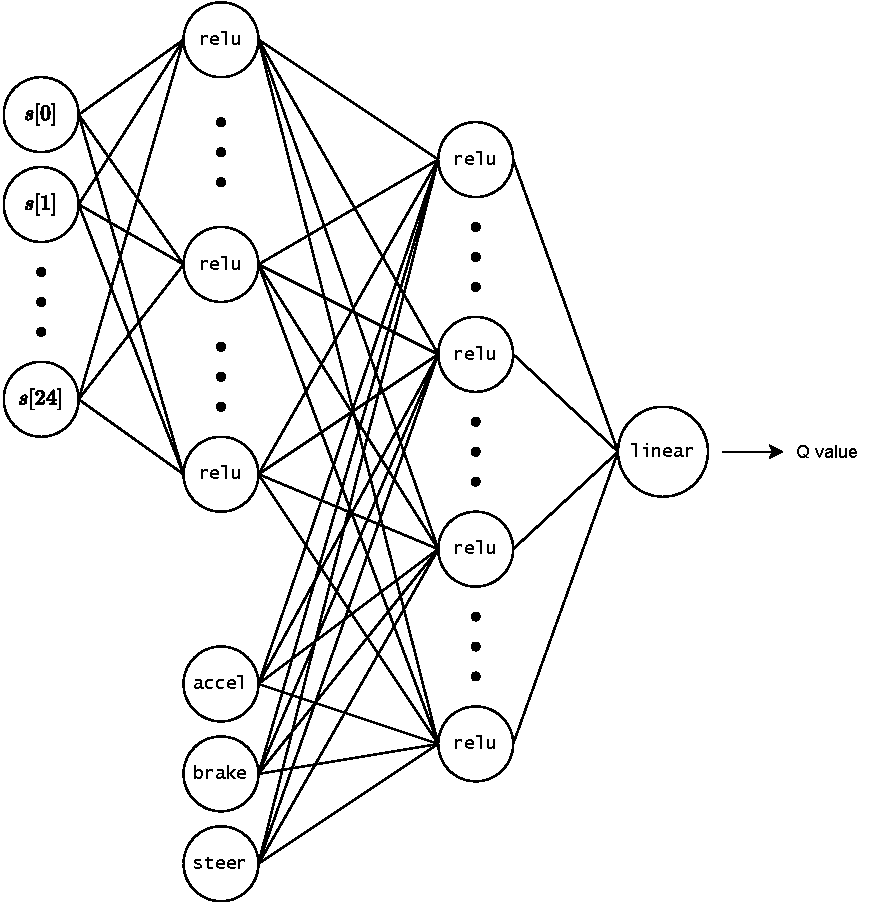
\includegraphics[width = 3.5in]{Figures/Chapter4/ddpg_critic_network.drawio.pdf}
    \caption{Rete Critic}
    \label{fig:critic_network}
\end{figure}

\clearpage

\section{Reward Shaping}

Come viene spiegato nel capitolo introduttivo del RL, la ricompensa è ciò che più di ogni altra cosa caratterizza l'apprendimento dell'agente. Essa infatti definisce \textit{cosa l'agente imparerà e come}.
\newline

L'obiettivo in questo caso è mantenere il veicolo al centro della corsia e terminare il percorso più velocemente possibile. La ricompensa sarà quindi funzione della velocità e dell'offset tra l'agente e il centro della corsia. Nella eq.\ref{rewardfunction} si definisce la funzione di ricompensa, dove le variabili sono definite nella tab. \ref{tab:statetable}.

\begin{equation}\label{rewardfunction}
r =
\begin{cases}
   S_x \, cos(\alpha) - |S_x \, sin(\alpha)| - |S_x \, \gamma| & \text{se } |\gamma|<1\\
   -200                                                        & \text{se } |\gamma|>1
\end{cases}
\end{equation}

con $S_x=speedX$, $\alpha=angle$ e $\gamma=trackPos$.
\newline

Oltre alla reward sopra definita sono state testate anche delle sue varianti. Una prima variante senza il controllo puntuale della trackPos, definita nella eq.\ref{rewardfunction_notrackpos}, e una sostituendo il controllo della trackPos con un controllo dell'angolo dell'auto rispetto alla carreggiata, definita nella eq.\ref{rewardfunction_angle}.

\begin{equation}\label{rewardfunction_notrackpos}
r =
\begin{cases}
   S_x \, cos(\alpha) - |S_x \, sin(\alpha)| & \text{se } |\gamma|<1\\
   -200                                      & \text{se } |\gamma|>1
\end{cases}
\end{equation}

\begin{equation}\label{rewardfunction_angle}
r =
\begin{cases}
   S_x \, cos(\alpha) - |S_x \, sin(\alpha)| - S_x\big|\frac{\alpha}{\pi}\big| & \text{se } |\gamma|<1\\
   -200                                                                        & \text{se } |\gamma|>1
\end{cases}
\end{equation}

\clearpage

\section{Rumore Esplorativo}

Negli algoritmi di Deep RL devono essere impostate strategie di esplorazione appropriate per evitare che l'algoritmo cada in un ottimo locale. Questo problema è comunemente noto come l'\textit{Explore-Exploit Dilemma}. 
\newline

\textit{L'Explore} consiste nella scelta di un'azione casuale. Ciò consente all'agente di migliorare le proprie conoscenze attuali sugli action-value, con un possibile vantaggio a lungo termine. 
Il miglioramento dell'accuratezza degli action-value stimati gli consentirà di prendere decisioni più informate in futuro. \textit{L'Exploit}, d'altra parte, sceglie l'azione avidamente per ottenere la massima ricompensa sfruttando le attuali stime delle action-value conosciute. 
Quando un agente esplora tende a costruire stime mano a mano più accurate degli action-value e quando sfrutta mira ad ottenere più ricompense. Non può, tuttavia, scegliere di fare entrambe le cose contemporaneamente. Per tale ragione è necessario utilizzare tecniche per la gestione delle fasi di esplorazione e sfruttamento.
\newline

In base all'algoritmo utilizzato esistono tecniche esplorative differenti. Nel caso del DQN, una nota strategia esplorativa è l'$\epsilon$-greedy, che consiste nell'eseguire un'azione casuale con probabilità $\epsilon$ e un'azione che massimizzi la $Q$ con probabilità $(1-\epsilon)$.
\newline

Strategie di esplorazione comuni come $\epsilon$-greedy non sono adatte a scenari di guida autonoma come quello esaminato in questa tesi perché si presenterebbero molti casi di azioni invalide, come ad esempio azioni in cui la frenata è maggiore dell'accelerazione.
\newline

Per tale ragione l'autore del DDPG propone l'utilizzo di un rumore additivo sull'azione generato dal processo stocastico di Ornstein-Uhlenbeck\cite{ddpgPaper}. Nell'ambito di questo lavoro sono stati testati tre tipi di rumori esplorativi: una variante dell'\textit{Ornstein-Uhlenbeck}, un \textit{Gaussian Noise} e un \textit{Time Variant Noise}. Questi rumori vengono presentati nelle seguenti sottosezioni.

\clearpage

\subsection{Ornstein-Uhlenbeck Mod}

Questo rumore è una variazione dell'\textit{Ornstein-Uhlenbeck} in quanto nel 10\% dei casi viene prodotto un rumore gaussiano $N(\mu,\sigma)$ mentre nel 90\% dei casi viene prodotto un rumore in base al classico processo stocastico di Ornstein-Uhlenbeck.
\newline

Questo serve a fare in modo che l'agente sia sollecitato con due stimoli molto diversi fra loro in misure diverse. Nove volte su dieci si stimola l'agente ad andare molto veloce attraverso un rumore additivo con media alta sull'accelerazione e nulla sulla frenata e, una volta su dieci, invece, lo si stimola a frenare attraverso un rumore con una media nettamente inferiore sull'accelerazione e alta sulla frenata.

\subsection{Gaussian Noise}

Questo rumore è una variazione dell'\textit{$\epsilon$-greedy Gaussian Noise} in quanto nel 90\% dei casi viene prodotto un rumore gaussiano $N(\mu_1,\sigma_1)$ mentre nel 10\% dei casi uno $N(\mu_2,\sigma_2)$. 
\newline

Anche in questo caso si utilizza questo stratagemma, con un opportuno tuning dei parametri di medie e std, per sollecitare l'agente con stimoli molto diversi fra loro per garantire che esso impari un più ampio spettro di comportamenti.
\newline

La probabilità $\epsilon$ viene fatta decadere linearmente rispetto al numero delle iterazioni di training.

\clearpage

\subsection{Time Variant Noise}

Il TVNoise è un rumore gaussiano con media e std variabile nel tempo.
La classe restituisce un rumore gaussiano $N(\mu_1,\sigma_1)$ per i primi \textbf{\texttt{time\_step1}} passi.
\newline

Successivamente tende linearmente ad un rumore con distribuzione gaussiana $N(\mu_2,\sigma_2)$ in un numero di passi pari a \\\textbf{\texttt{(self.time\_step2 - self.time\_step1)}}.
\newline

Infine, sempre linearmente, tende a $N(\mu_3,\sigma_3)$ in \textbf{\texttt{(self.time\_step3 - self.time\_step2)}} passi. Nel progetto di tesi questo terzo passaggio viene sfruttato per far decadere a zero linearmente il rumore gaussiano aggiunto.
\newline

Nella fig.\ref{fig:tv_noise_media} viene mostrato un esempio di possibile andamento della media del rumore gaussiano. Lo stesso ragionamento si applica alla std.

\begin{figure}[hb]
    \center
    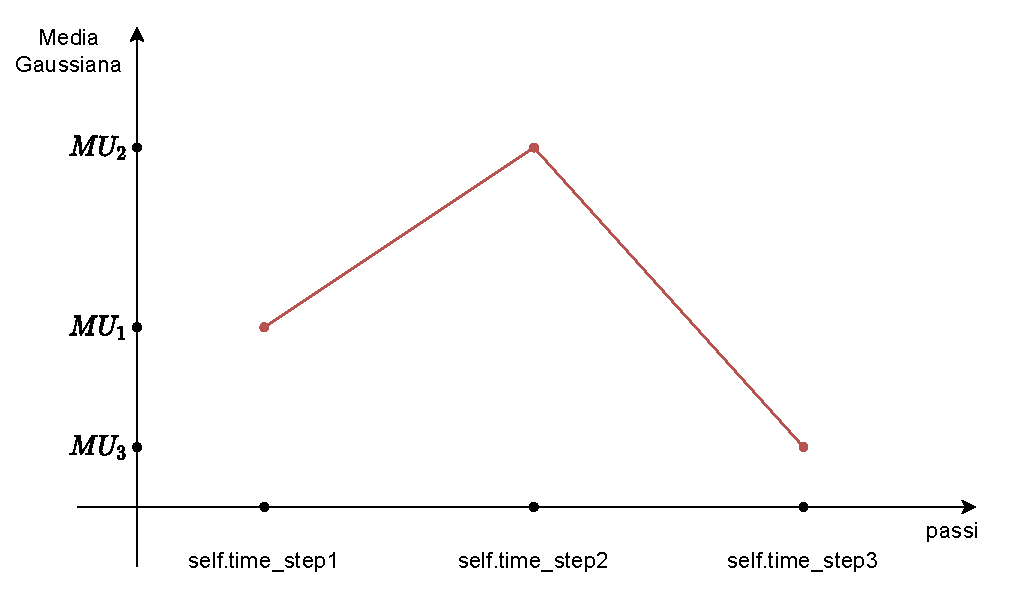
\includegraphics[width = 5in]{Figures/Appendix/tvnoise_media.drawio.pdf}
    \caption{Andamento della media Gaussiana}
    \label{fig:tv_noise_media}
\end{figure}